% !TeX spellcheck = en_GB

\section{Vertical SWC - all ensemble member}%\hfill} 
\label{app:vert_ensmemb09}

%%% image ensemble spread %%%%%%%%%%%%%%%%%%%%%%%%%%%%%%%%%%%%%
\begin{figure}[h]%\ContinuedFloat
	\centering
	% 21/12
	\begin{subfigure}[t]{\textwidth} 
		\centering
		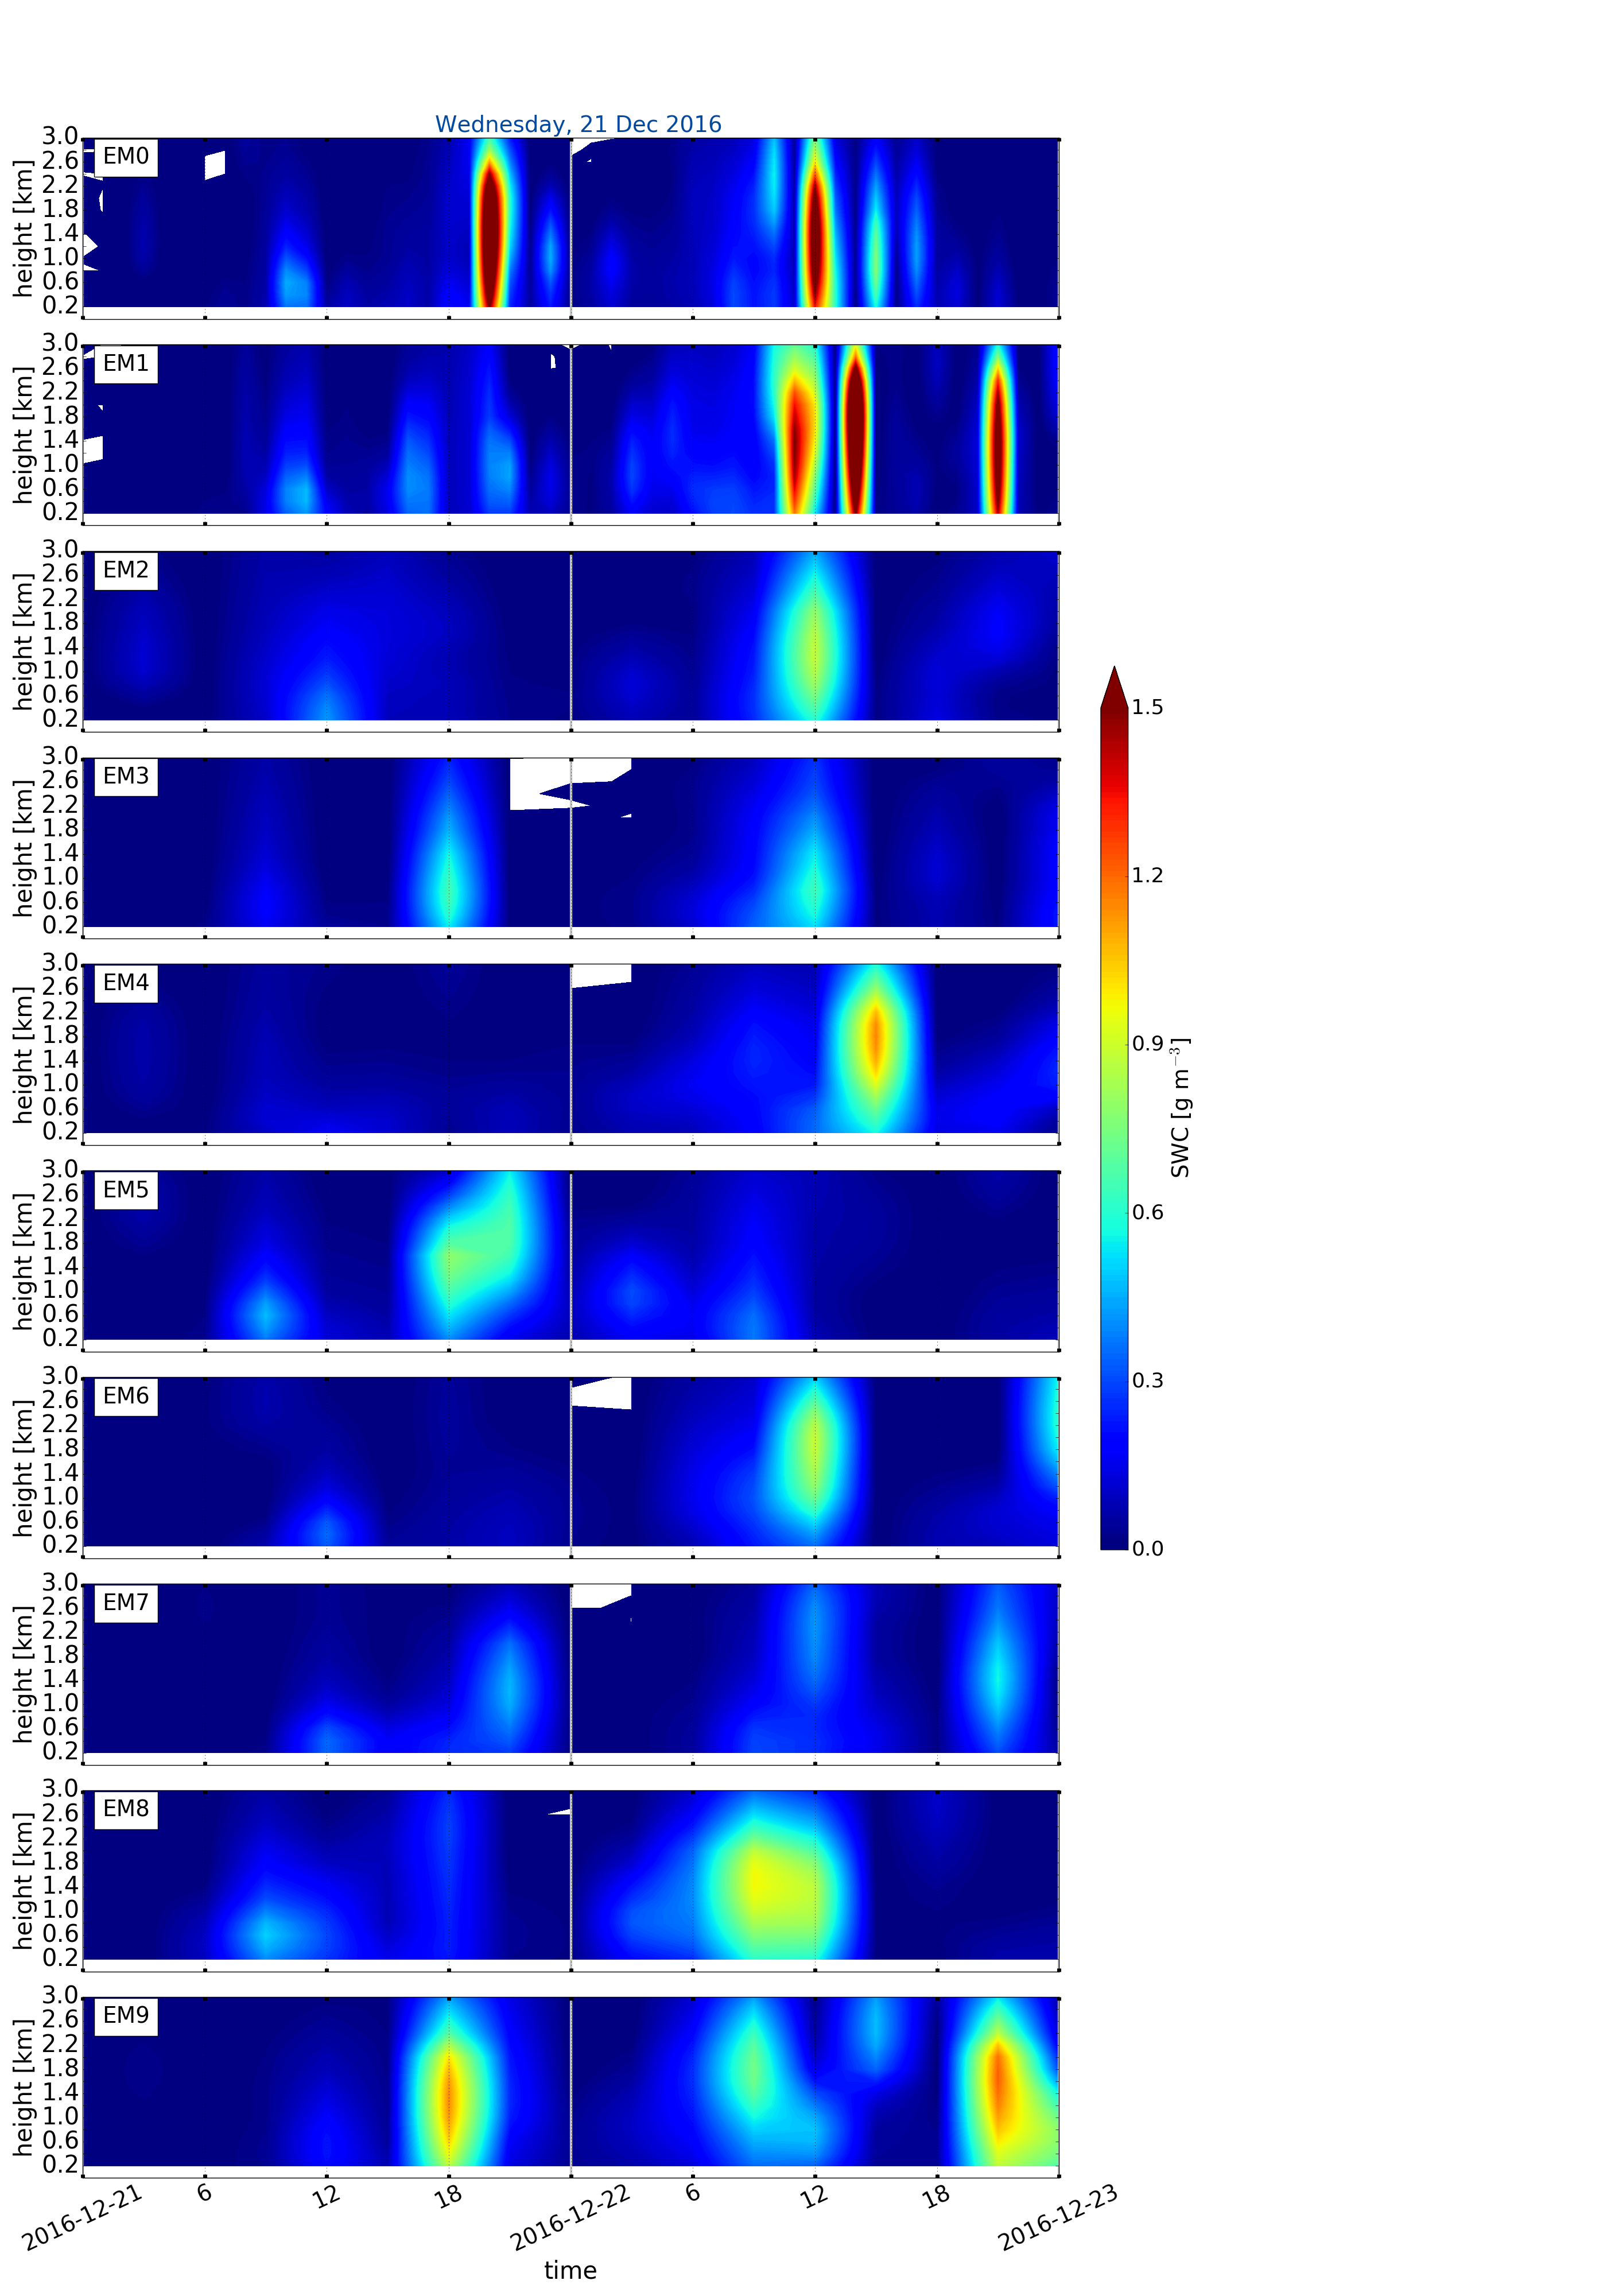
\includegraphics[trim={0cm 0cm 18.3cm 5.1cm},clip,width=0.8\textwidth]{./fig_09EM/20161221}
		\caption{}\label{fig:EM09_21}
	\end{subfigure}
    \caption{Vertical SWC of each individual ensemble member from \numrange{0}{9} forecast for \SI{48}{\hour}. Initialised \SI{21}{\dec} at \SI{0}{\UTC}.}\label{fig:EM09}
\end{figure}
\begin{figure}[h]\ContinuedFloat
	\centering
	% 22/12
	\begin{subfigure}[t]{\textwidth} 
		\centering
		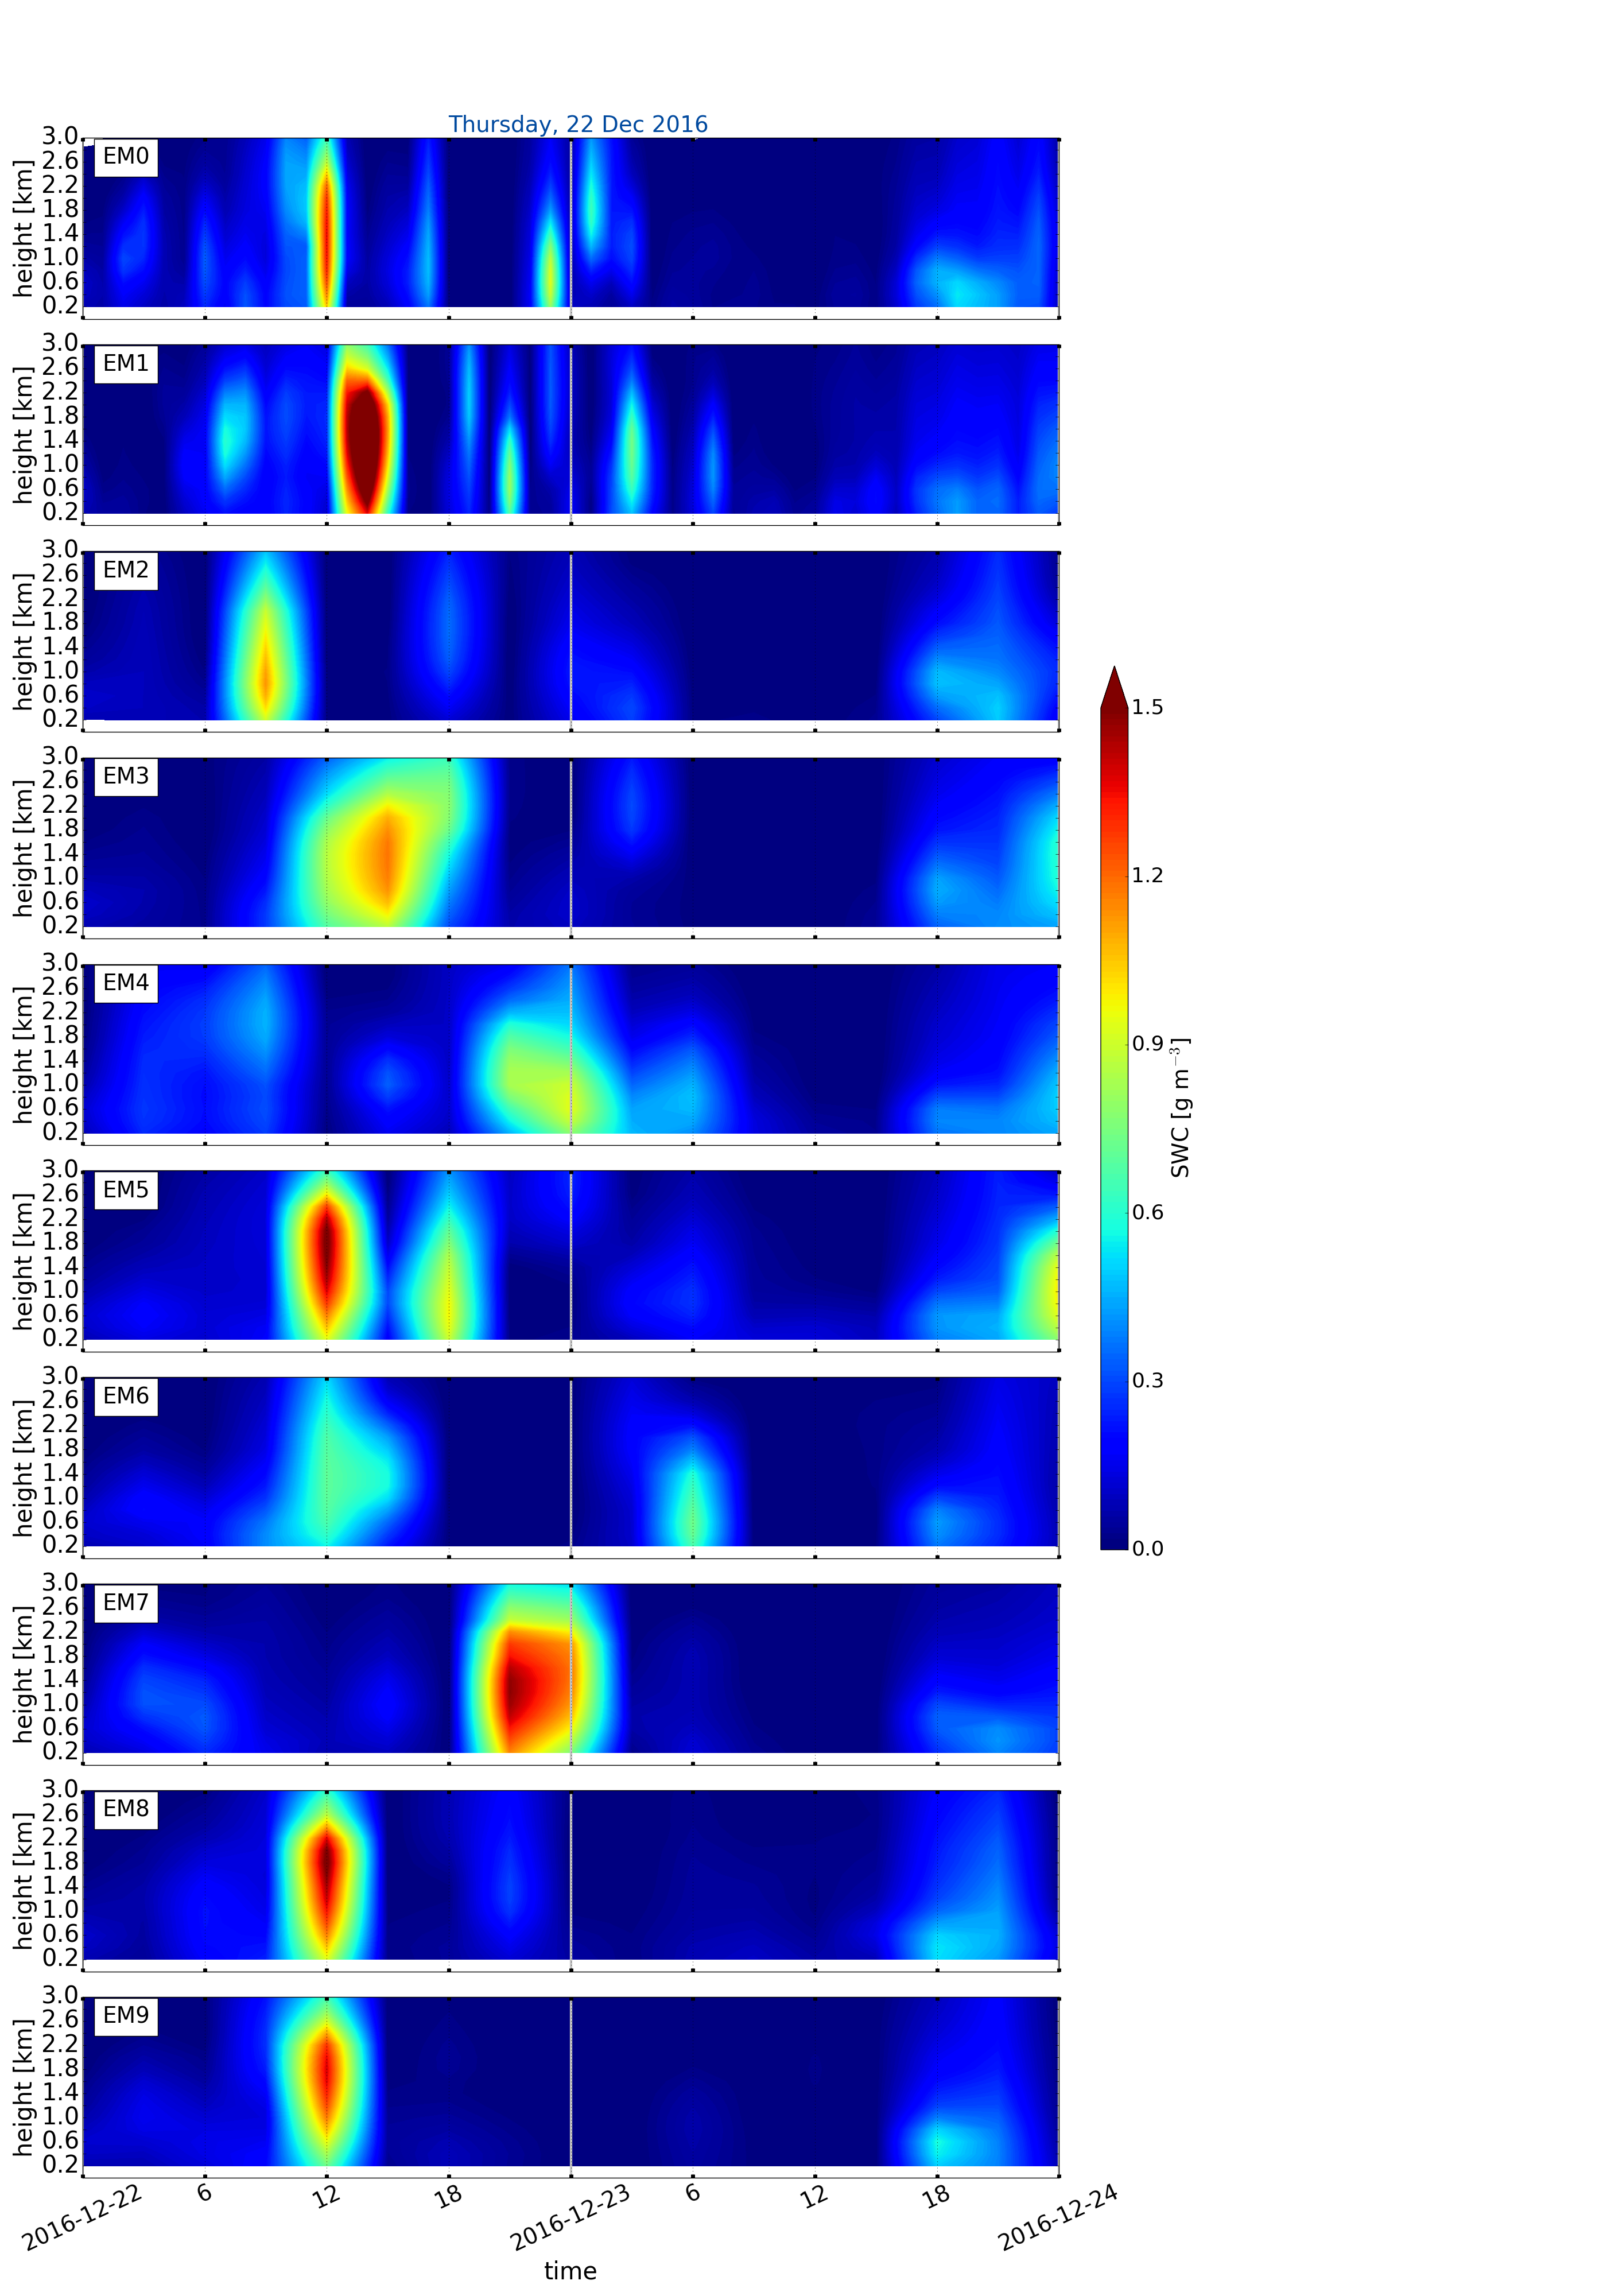
\includegraphics[trim={0cm 0cm 18.3cm 5.1cm},clip,width=0.8\textwidth]{./fig_09EM/20161222}
		\caption{}\label{fig:EM09_22}
	\end{subfigure}
    \caption{\textit{(Continued from previous page.)} Initialised \SI{22}{\dec} at \SI{0}{\UTC}. } 
\end{figure}
\begin{figure}\ContinuedFloat
	\centering
	% 23/12
	\begin{subfigure}[t]{\textwidth} 
		\centering
		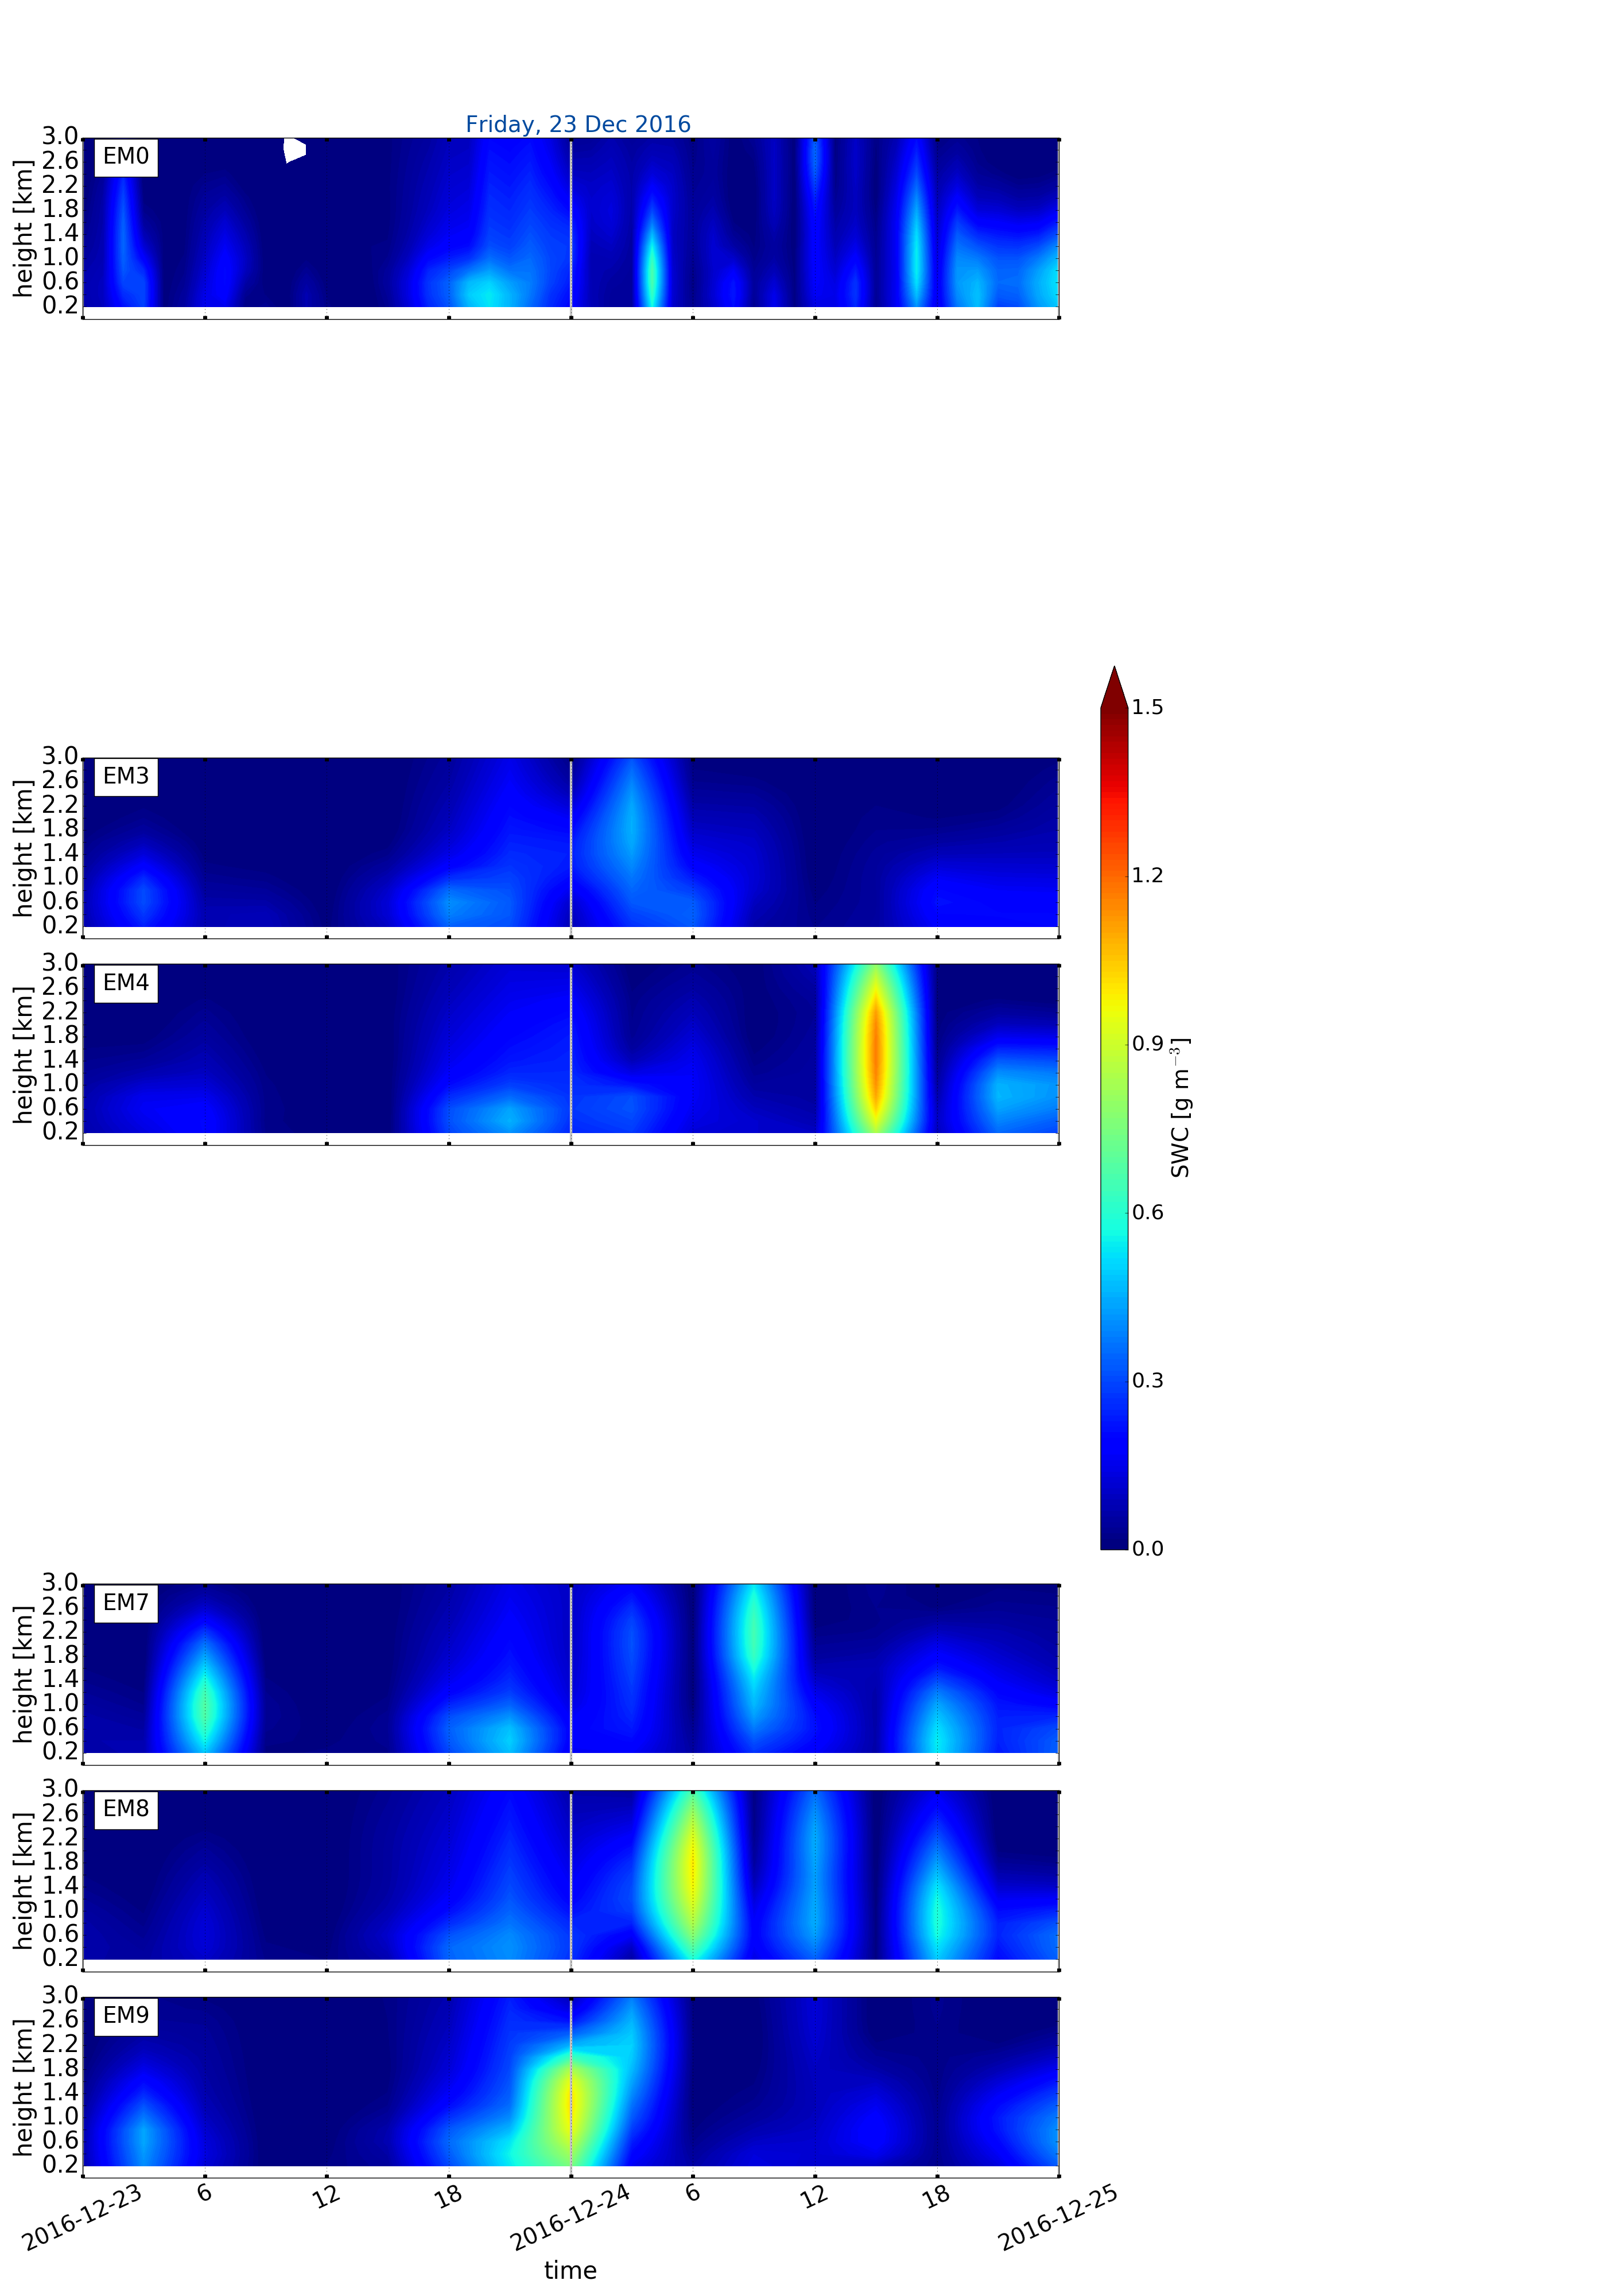
\includegraphics[trim={0cm 0cm 18.3cm 5.1cm},clip,width=0.8\textwidth]{./fig_09EM/20161223}
		\caption{}\label{fig:EM09_23}
	\end{subfigure}
    \caption{\textit{(Continued from previous page.)} Initialised \SI{23}{\dec} at \SI{0}{\UTC}. } 
\end{figure}
\begin{figure}\ContinuedFloat
	\centering
			\begin{subfigure}[t]{\textwidth}
            \centering
            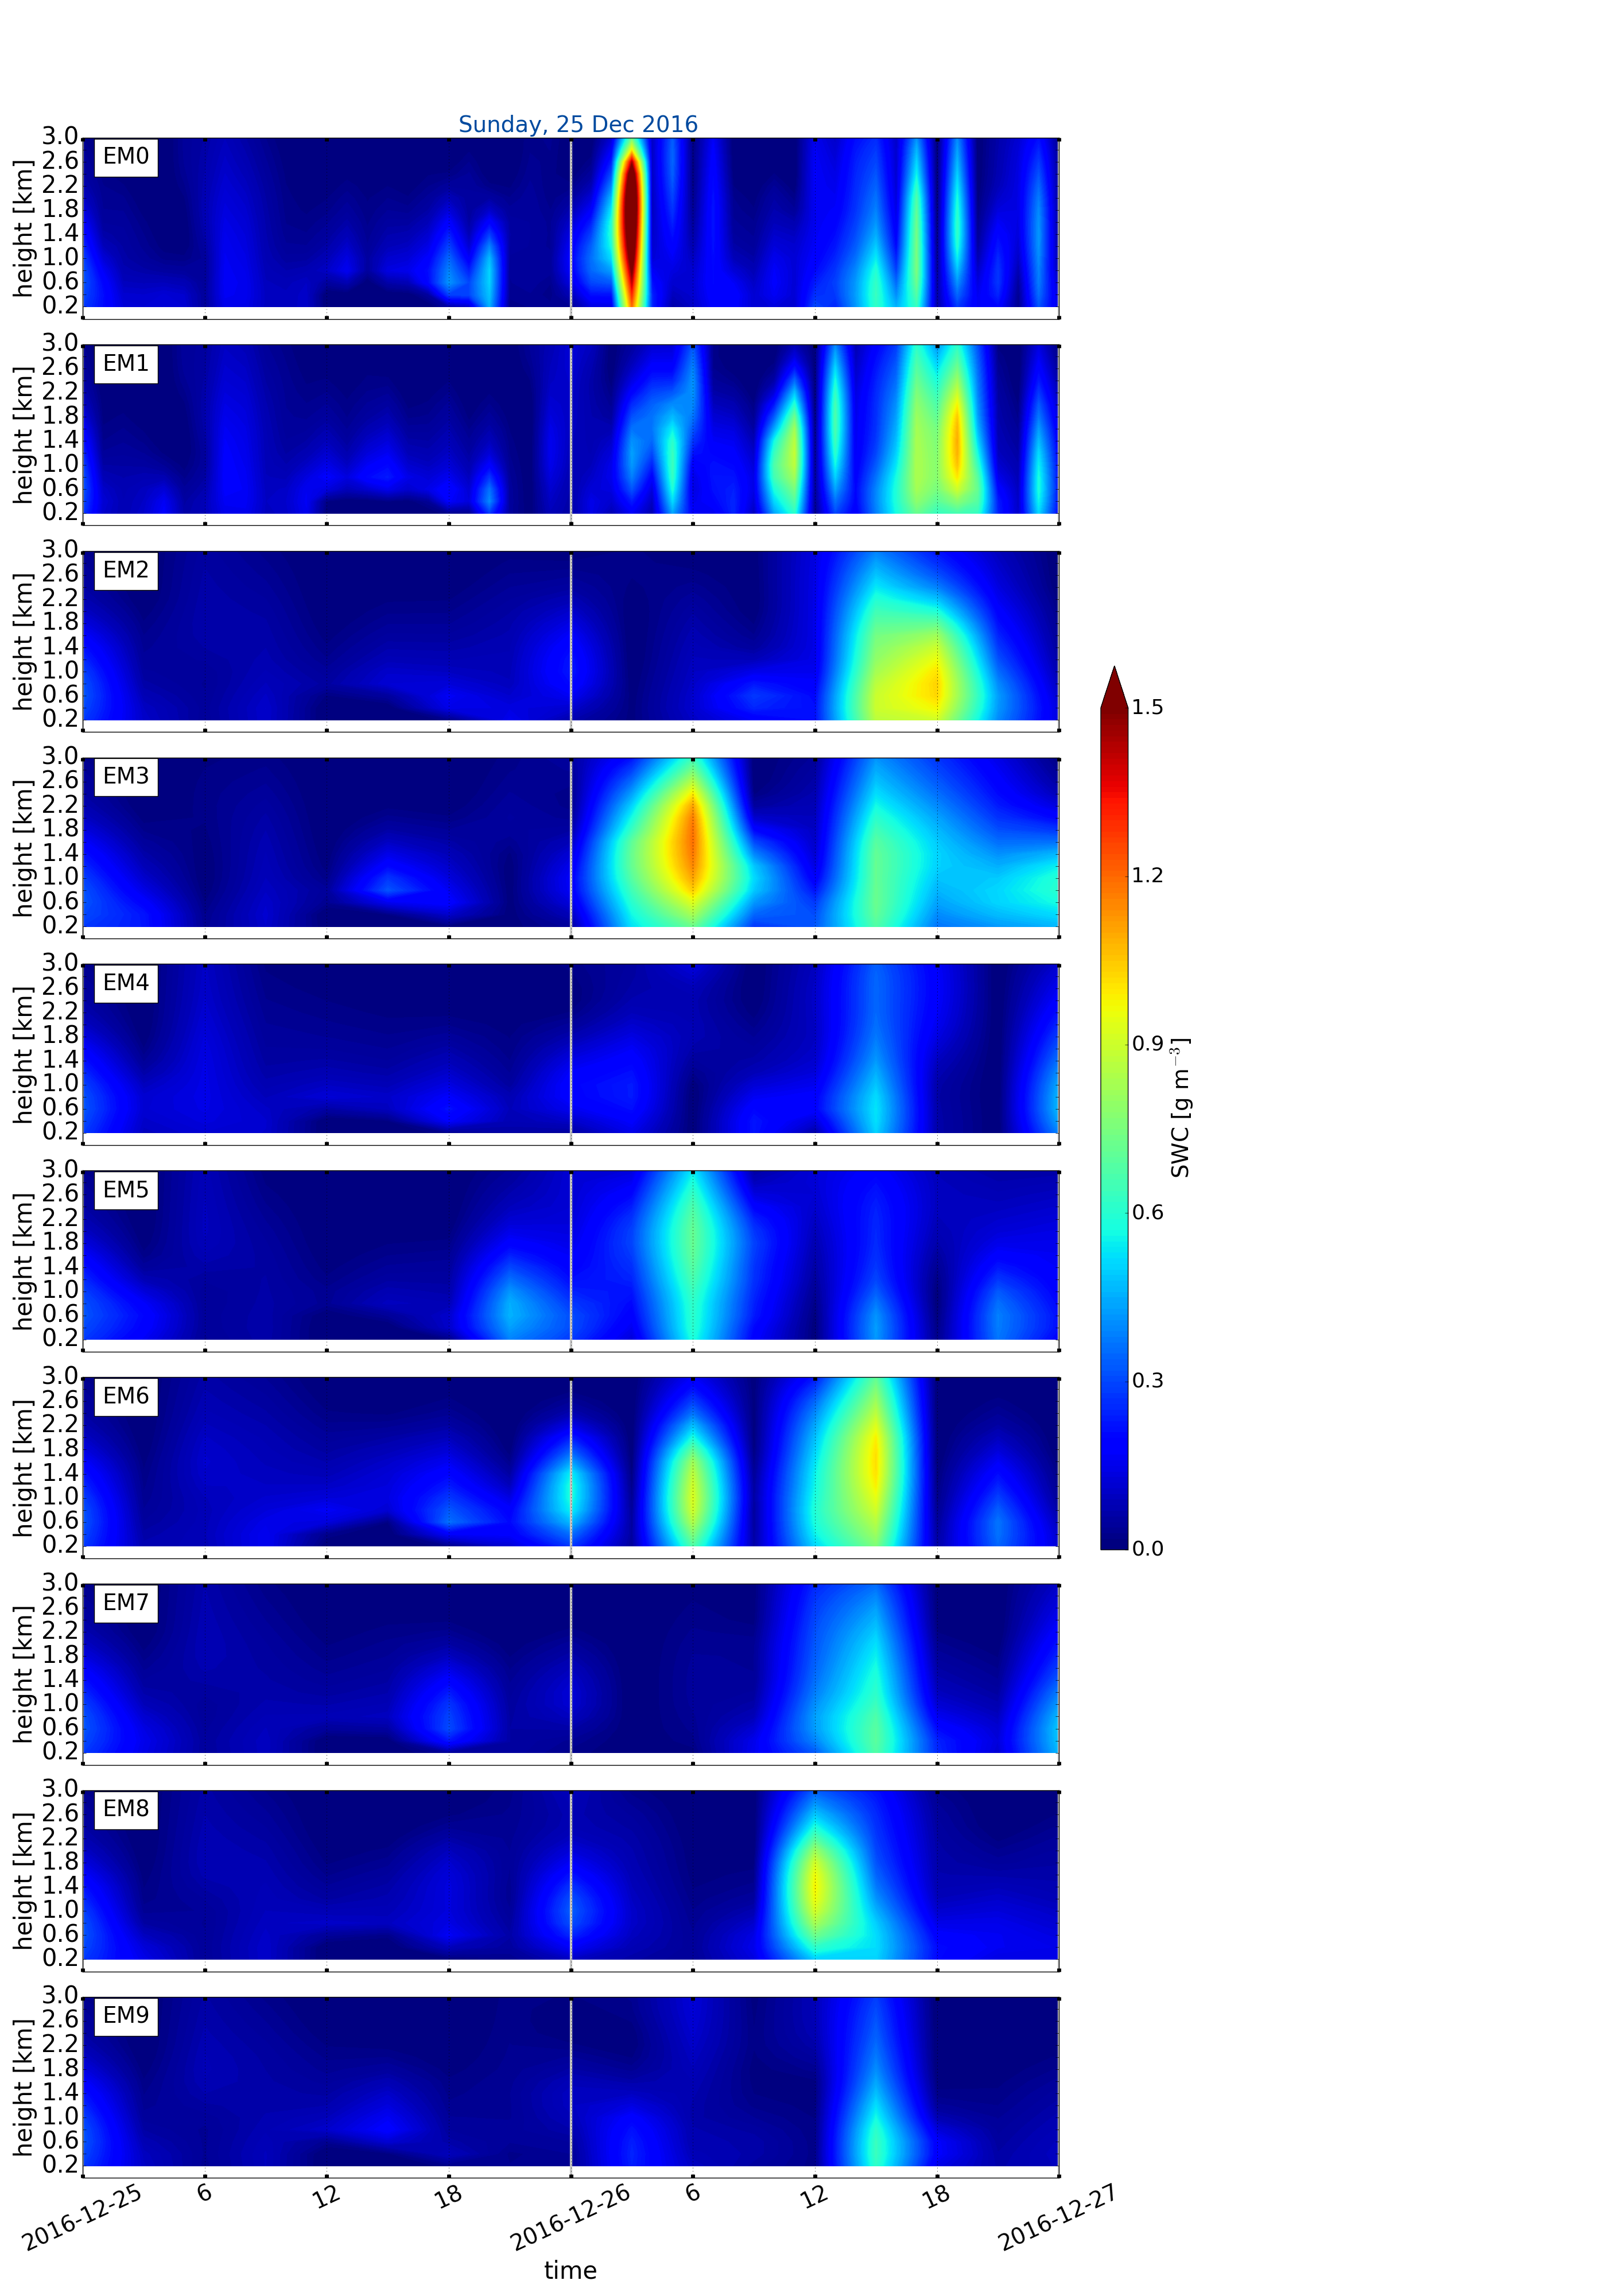
\includegraphics[trim={0cm 0cm 18.3cm 5.1cm},clip,width=0.8\textwidth]{./fig_09EM/20161225}
				\caption{}\label{fig:EM09_25}
			\end{subfigure}
    \caption{\textit{(Continued from previous page.)} Initialised \SI{25}{\dec} at \SI{0}{\UTC}. }        
\end{figure}
\begin{figure}[t]\ContinuedFloat
	\centering
	% 26/12
	\begin{subfigure}[t]{\textwidth}	
		\centering
		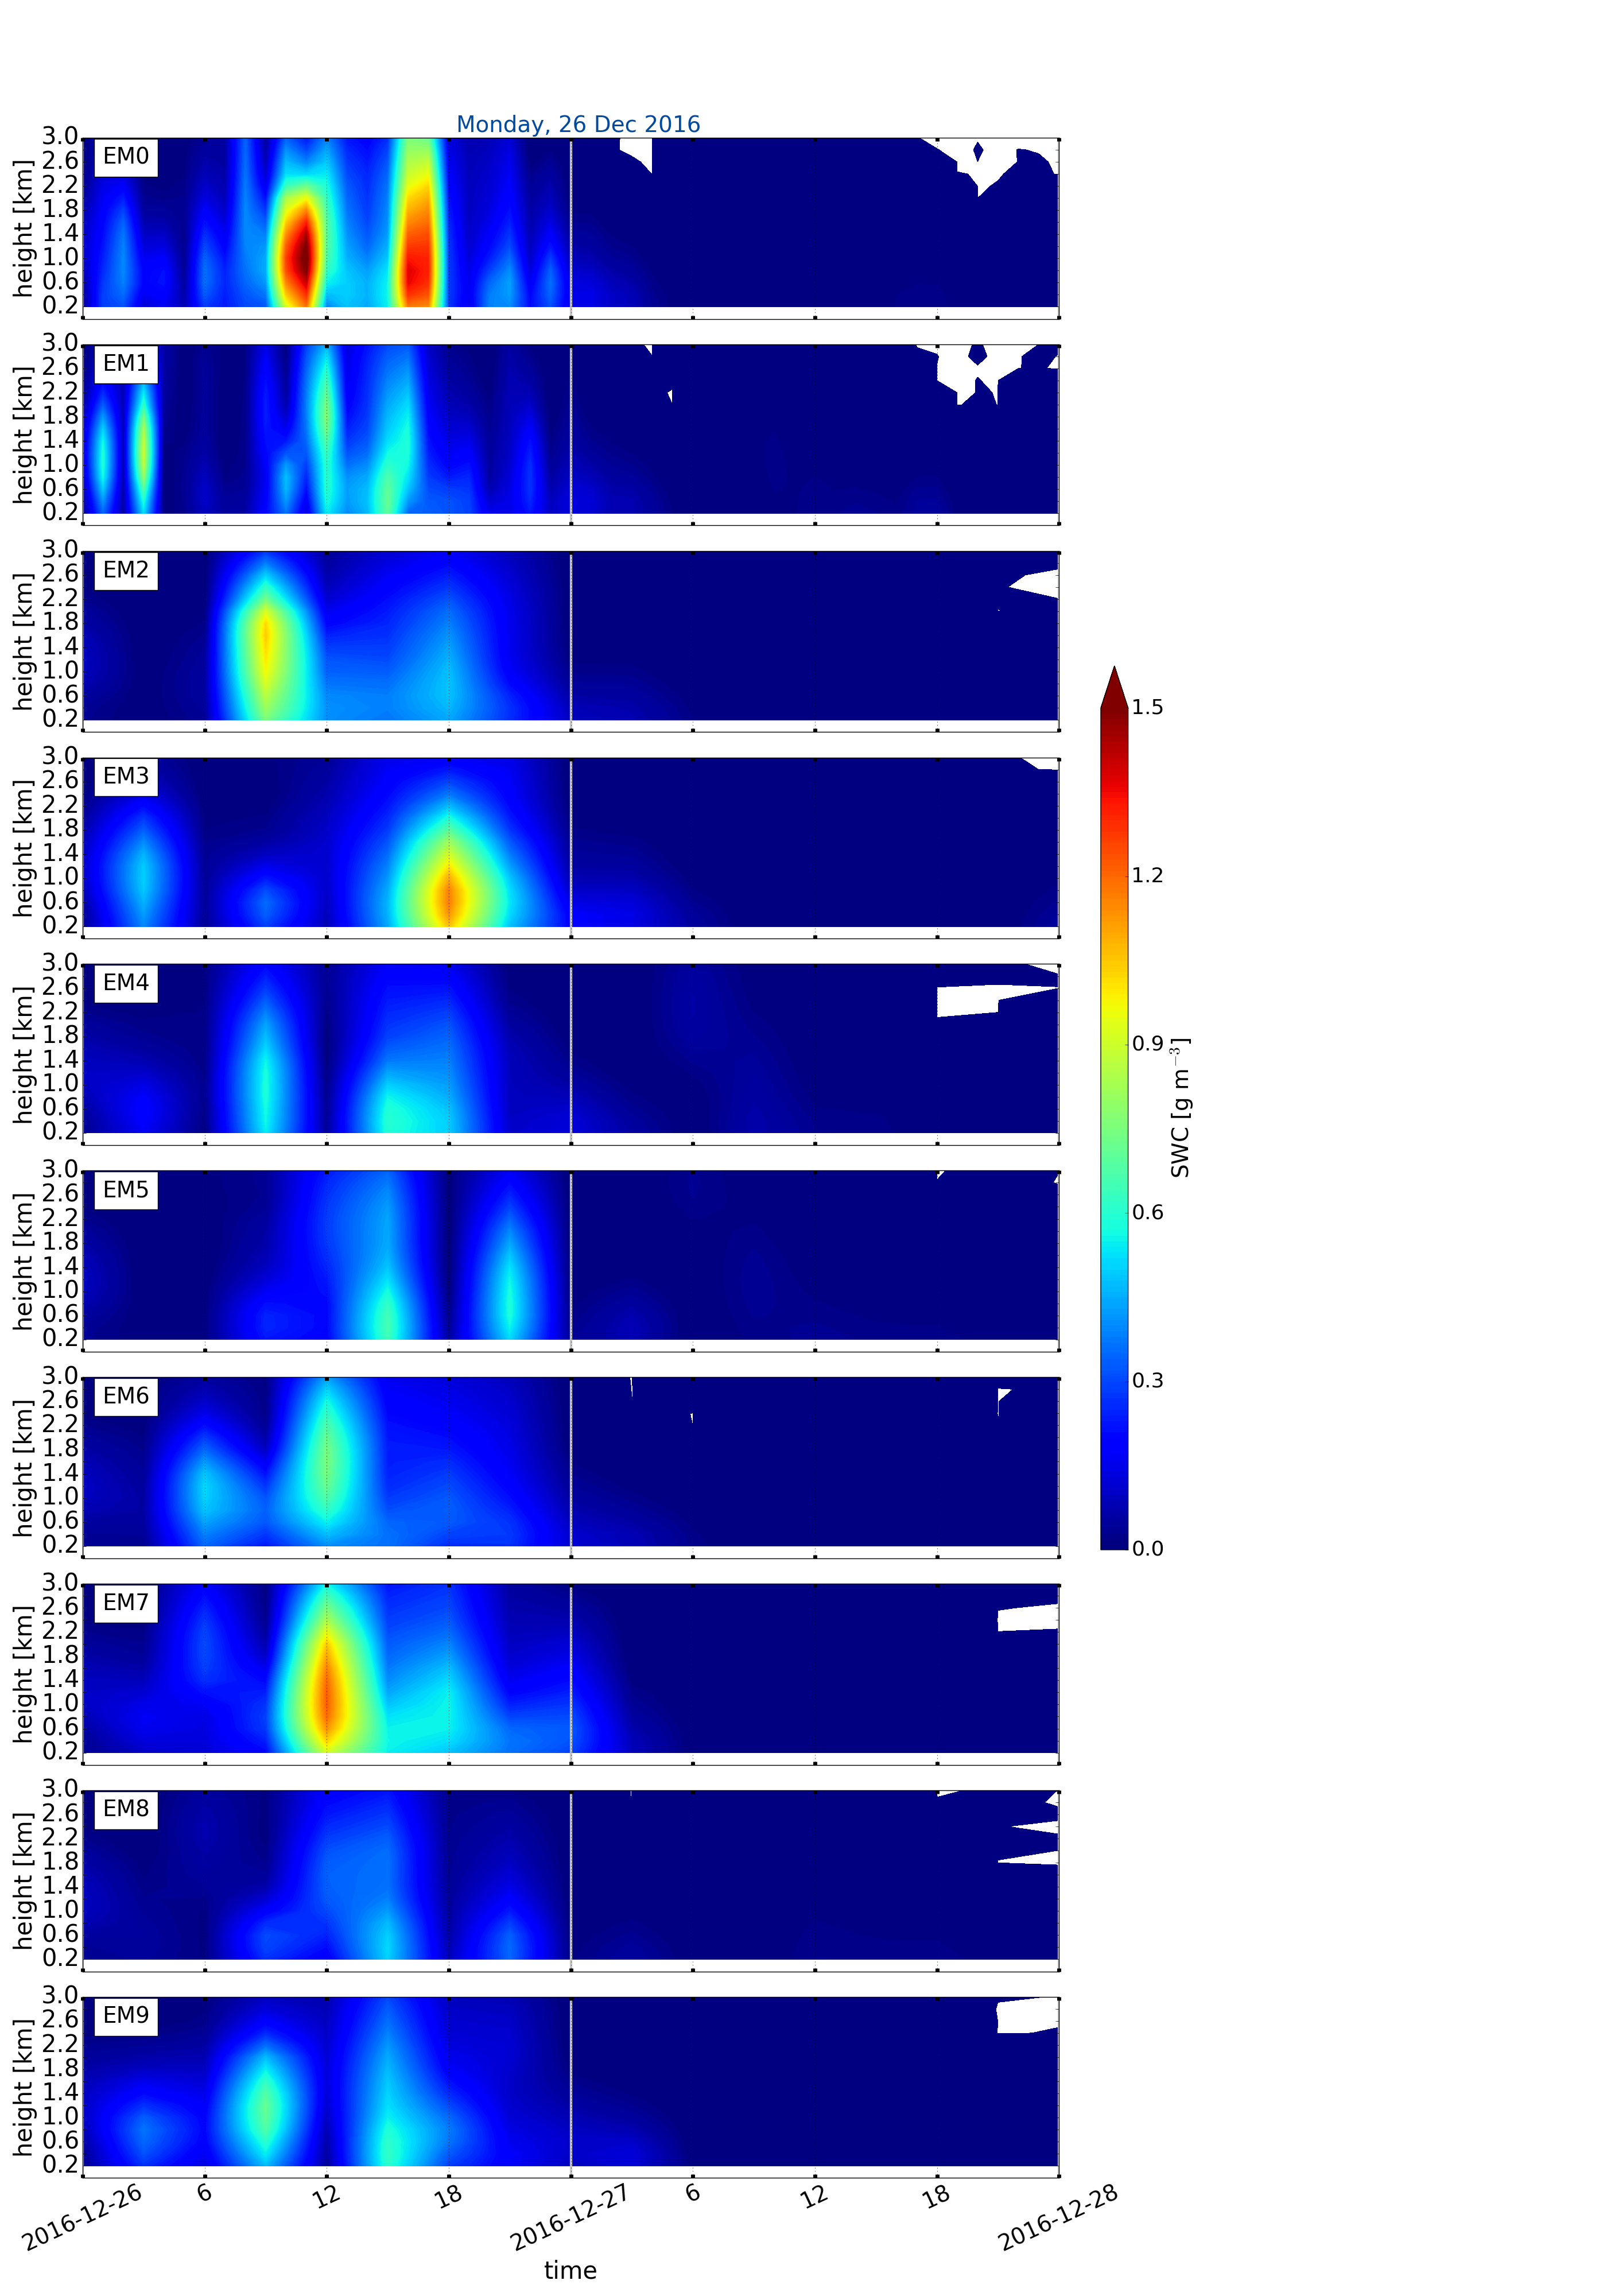
\includegraphics[trim={0cm 0cm 18.3cm 5.1cm},clip,width=0.8\textwidth]{./fig_09EM/20161226}
		\caption{}\label{fig:EM09_26}
	\end{subfigure}
	\caption{\textit{(Continued from previous page.)} Initialised \SI{26}{\dec} at \SI{0}{\UTC}.}
\end{figure}

%%%%%%%%%%%%%%%%%%%%%%%%%%%%%%%%%%%%%%%%%%%%%%%%%%%%%%%%%%%%%%%%%%%%%%%%%%
